\section{Einarbeitung}
In der Einarbeitungsphase haben wir uns zunächst für eine Hadoop-Arbeitsumgebung entschieden. Da die meisten Projektteilnehmer über lediglich vier Gigabyte Arbeitsspeicher verfügen, fiel unsere Wahl auf die ressourcenschonende Hortonworks Sandbox \footnote{Siehe: \url{http://hortonworks.com/products/hortonworks-sandbox/}}, die bei allen Teilnehmern problemlos ausgeführt werden konnte. Unter Verwendung der Sandbox haben wir den Umgang mit dem Hadoop-Ecosystem gelernt und erste Map/Reduce-Jobs ausgeführt. Darüber hinaus konnten wir weitere Tools wie Hive und Pig verwenden.

\subsection{Datenmodell}
Abbildung \ref{fig:ShoppersTables} zeigt das Datenmodell, dass aus den Entitäten transactions, history, offers, und submissions besteht. 

\begin{figure}[h]
\centering
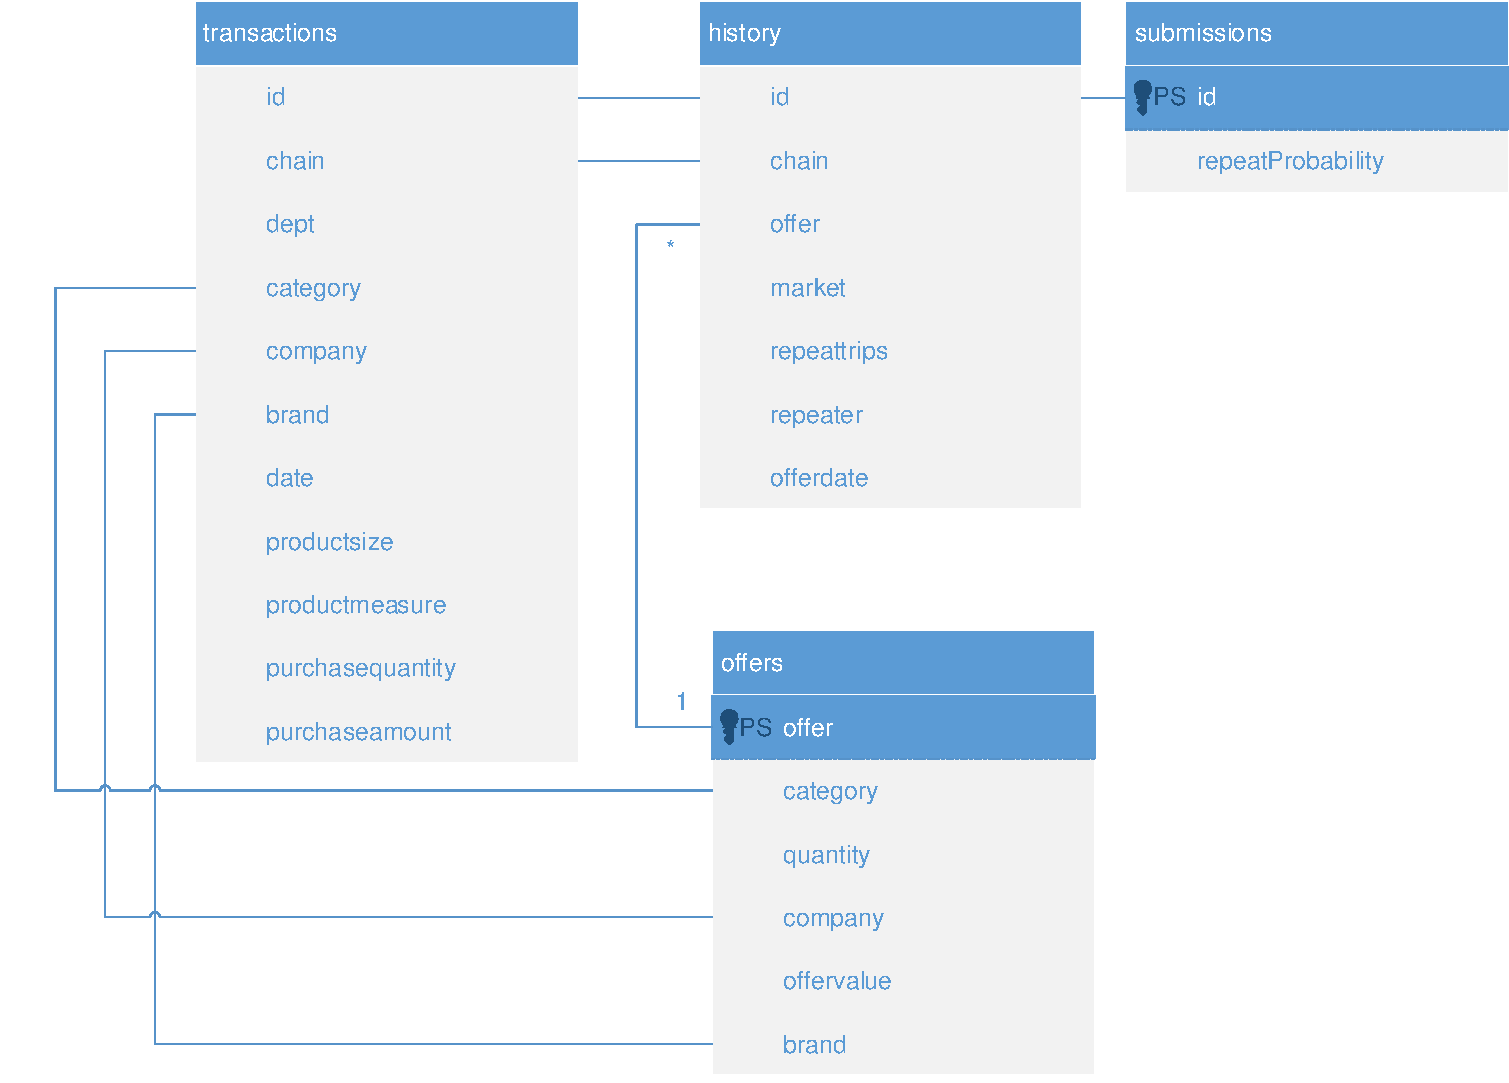
\includegraphics[width=0.7\linewidth]{Bilder/ShoppersTables}
\caption{Das Datenmodell der Shoppers-Challenge}
\label{fig:ShoppersTables}
\end{figure}

In der Tabelle \textbf{transactions} stehen die Einkäufe der Kunden:\\
\begin{tabular}{|l|l|}
	\hline \textbf{Feld} & \textbf{Bedeutung}  \\ 
	\hline id & ID des Kunden \\ 
	\hline chain & ID der Marktkette \\ 
	\hline dept  & ID der Produktoberkategorie (z.B. Elektronikgeräte)  \\ 
	\hline category & ID der Produktkategorie (z.B. Smartphones) \\ 
	\hline company & ID der Firma die das Produkt verkauft \\ 
	\hline brand & ID der Marke (z.B. iPhone) \\ 
	\hline date & Kaufdatum \\
	\hline productsize & Menge die gekauft wurde (2L Wasser, 500g Mehl) \\ 	
	\hline productmeasure & Einheit (Liter, Gramm, Stück) \\ 	
	\hline purchasequantity & Stückzahl die gekauft wurde (Drei 2L Flaschen Wasser) \\ 
	\hline purchaseamount & Preis in Dollar \\ 
	\hline 
\end{tabular}

Die Tabelle \textbf{offers} beschreibt Coupons, die den Kunden angeboten wurden:\\
\begin{tabular}{|l|l|}
	\hline \textbf{Feld} & \textbf{Bedeutung}  \\ 
	\hline offer & ID des Coupon \\ 
	\hline category & ID der Produktkategorie \\ 
	\hline quantity & Stückzahl ab der ein Coupon gilt \\ 
	\hline company & ID der Firma die Coupons anbietet \\ 
	\hline offervalue & Preis \\ 
	\hline brand & ID der Marke \\ 
	\hline 
\end{tabular}

Die Tabelle \textbf{train\_history} enthält Informationen darüber, wann den Kunden die Coupons angeboten wurden: \\
\begin{tabular}{|l|l|}
	\hline \textbf{Feld} & \textbf{Bedeutung}  \\ 
	\hline id & ID des Kunden \\ 
	\hline chain & ID der Marktkette \\ 
	\hline offer  & ID des Coupon  \\ 
	\hline market & ID der Region in der sich der Markt befindet  \\ 
	\hline repeattrips & Anzahl der Wiederholungskäufe (gleiches Produkt)  \\ 
	\hline repeater & Gibt an, ob repeattrips größer 0 ist \\ 
	\hline offerdate & Datum an dem der Kunde den Coupon erhalten hat \\ 
	\hline 
\end{tabular} 

Die Tabelle \textit{test\_history} entspricht der Tabelle \textit{train\_history} mit dem Unterschied, dass die beiden Felder \textit{repeattrips} und \textit{repeater} fehlen. Diese sind absichtlich nicht enthalten, da eine Vorhersage über diese Werte getroffen werden soll.


Die Tabelle \textbf{submissions} enthält die Ergebnisse, die wir bei Kaggle einreichen:\\
\begin{tabular}{|l|l|}
	\hline \textbf{Feld} & \textbf{Bedeutung}  \\ 
	\hline id & ID des Kunden \\ 
	\hline repeatProbability & Wahrscheinlichkeit das der Kunde erneut kauft \\ 
	\hline 
\end{tabular} 




\subsection{Technologieentscheidung}
Zu Beginn des Projekts haben wir uns Gedanken über die Auswahl der Technologien gemacht. Zum Zeitpunkt der Einarbeitungsphase haben wir bereits Hive und Pig durch gruppenübergreifende Vorträge kennen gelernt. Darüber hinaus standen uns keine weiteren Optionen zur Verfügung, da alternative Technologien erst zu einem späteren Zeitpunkt vorgestellt worden sind.

Somit beschränkte sich die Technologieentscheidung auf die Wahl zwischen Hive und Pig. Da wir in unserem Projekt ausschließlich Analysen auf strukturierte Daten durchgeführt haben, fiel unsere Entscheidung auf Hive. Der einfache Datenimport in Form von Tabellen und die einfachen Abfragemöglichkeiten in der SQL ähnlichen Abfragesprache HQL waren die ausschlaggebenden Kriterien.

Die Technologien, die wir neben Hive verwendet haben, werden im weiteren Verlauf der Dokumentation erläutert.


\subsection{Data-Mining-Verfahren}
